First we report the speedups and energy saving achieved on two architectures applying
loop optimizations. Then we show loop optimizations that work the best on
one architecture do not necessarily work the best on the other, in terms of
time taken and energy consumed.
\subsection{Speedups and Energy Savings}

\begin{table}
  \centering{
\caption{Time and Energy Comparison of Optimal Configuration to Baseline of Polybench Kernels}
\begin{tabular}{ |l|c|c|c|c| }
  \hline
  \multirow{2}{*}{\textbf{Benchmark}} & \multicolumn{2}{|c|}{\textit{Time}} & \multicolumn{2}{|c|}{\textit{Energy}} \\
  \cline{2-5}
  & SM & LG & SM & LG \\
  \hline
  2mm & 1.48X & 1.36X & 1.28X & \textcolor{red}{0.77X} \\
  \hline
  covariance & 37.86X & 122.20X & 25.11X & 60.31X \\
  \hline
  gemm & 1.46X & 1.44X & 1.28X & \textcolor{red}{0.78X} \\
  \hline
  gramschmidt & 19.41X & 21.64X & 13.66X & 11.72X \\
  \hline
  jacobi-2d & 1.31X & 1.48X & 1.37X & 1.44X \\
  \hline
  seidel-2d & 7.76X & 9.60X & 7.68X & 5.53X \\
  \hline
\end{tabular}
}
\end{table}

\subsection{Cross Architecture Comparsion}

\begin{figure}
\centering
\subfigure[Best SandyBridge Optimization Sequences on Xeon Phi] {                        
  %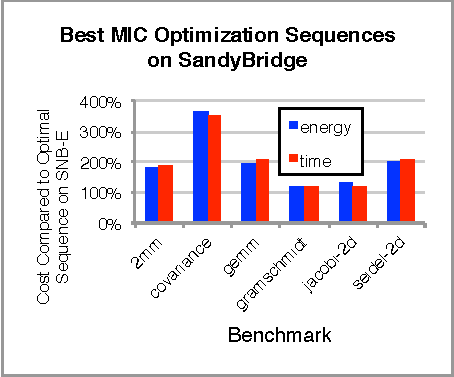
\includegraphics[width=0.45\textwidth]{BestMIConSNB}   
  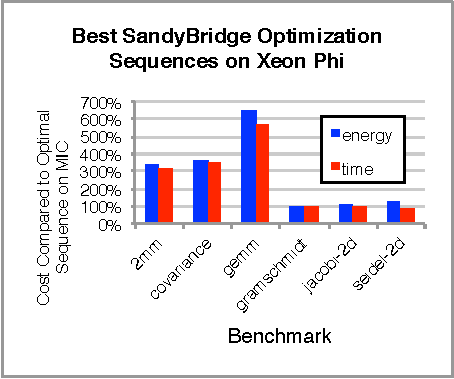
\includegraphics{BestSNBonMIC}
  \label{Sandy}
} 
\subfigure[Best MIC Optimization Sequences on SandyBridge] {               
  %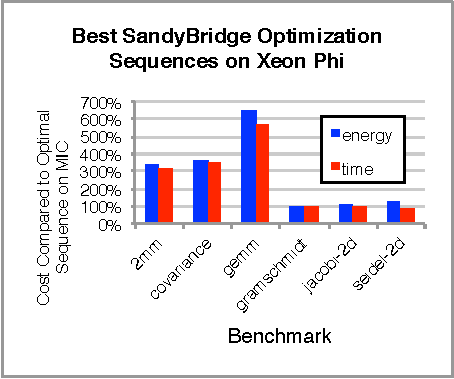
\includegraphics[width=0.45\textwidth]{BestSNBonMIC}
  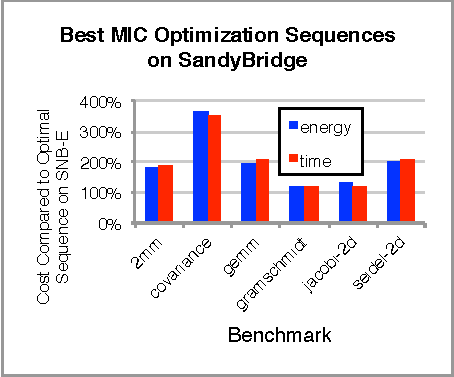
\includegraphics{BestMIConSNB}   
  \label{MIC}
} 
\caption{
}                   
\label{fig:Brdr2d-TE}                                                   
\end{figure} 

Figure~\ref{Sandy} shows the best optimization sequences of the six benchmarks
chosen from Sandy Bridge do not perform as good when run on the MIC architecture. 
Comparing with the optimal optimization sequence on the MIC, the Sandy Bridge
sequences incurred significant increase in execution time and energy consumption
for 2mm, covariance, and gemm. The Sandy Bridge optimization sequences 
performed as good as the optimal sequence on the MIC for the other three benchmarks. 
Figure~\ref{MIC} compares the time and energy (running on Sandy Bridge) of 
the best optimization sequences chosen from MIC with those of the optimal optimization 
sequences chosen from Sandy Bridge. 2mm, covariance, gemm, and seidel-2d consumed
from ~200\% to ~350\% more energy and time. 
